% A countable transitive inner model M sitting inside the universe V,
% with M's cardinals ℵ_1^M, ℵ_2^M below V's, collapsed by a function f.
% Source: book/tex/set-theory/models.tex (§ Picturing inner models).
\documentclass[border=2mm]{standalone}
\usepackage{tikz}
\usepackage{amssymb}
\usetikzlibrary{arrows.meta}
\begin{document}
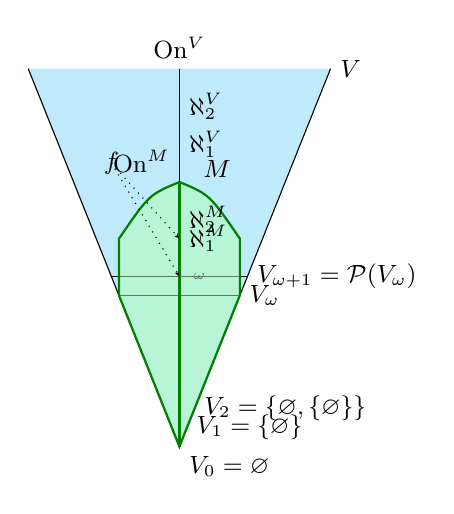
\begin{tikzpicture}[scale=0.16, every node/.style={font=\small}]
  \fill[cyan!25] (0,0) -- (12,30) -- (-12,30) -- cycle;
  \draw (12,30) -- (0,0) -- (-12,30);
  \node[right] at (12,30) {$V$};
  \node[below right] at (0,0) {$V_0 = \varnothing$};
  \node[right] at (0.6,1.5) {$V_1 = \{\varnothing\}$};
  \node[right] at (1.2,3) {$V_2 = \{\varnothing, \{\varnothing\}\}$};
  \draw (-4.8,12) -- (4.8,12) node[right] {$V_\omega$};
  \draw (-5.4,13.5) -- (5.4,13.5) node[right] {$V_{\omega+1} = \mathcal{P}(V_\omega)$};
  \node[right] at (0.3,13.5) {\tiny $\omega$};
  % inner model M (green sub-triangle, apex bulging to 0.7*On)
  \fill[green!30, opacity=0.5] (0,0) -- (4.8,12) -- (4.8,16.5)
      .. controls (2.4,20) .. (0,21) .. controls (-2.4,20) .. (-4.8,16.5) -- (-4.8,12) -- cycle;
  \draw[green!50!black, thick] (0,0) -- (4.8,12) -- (4.8,16.5)
      .. controls (2.4,20) .. (0,21) .. controls (-2.4,20) .. (-4.8,16.5) -- (-4.8,12) -- cycle;
  \node at (3,22) {$M$};
  % axes
  \draw (0,0) -- (0,30);
  \draw[green!50!black, thick] (0,0) -- (0,21);
  \node[above] at (0,30) {$\mathrm{On}^V$};
  \node[above left] at (0,21) {$\mathrm{On}^M$};
  % cardinals
  \node[right] at (0,24) {$\aleph_1^V$};
  \node[right] at (0,27) {$\aleph_2^V$};
  \node[right] at (0,16.5) {$\aleph_1^M$};
  \node[right] at (0,18) {$\aleph_2^M$};
  % collapsing function f
  \node at (-5.4,22.5) {$f$};
  \draw[dotted, -{Stealth[length=2pt]}] (-5.4,22.5) -- (0,16.5);
  \draw[dotted, -{Stealth[length=2pt]}] (-5.4,22.5) -- (0,13.5);
\end{tikzpicture}
\end{document}
